% Chapter 1

\chapter{Introduction} % Main chapter title

\label{Chapter1} % For referencing the chapter elsewhere, use \ref{Chapter1} 

%----------------------------------------------------------------------------------------

% Define some commands to keep the formatting separated from the content 
\newcommand{\keyword}[1]{\textbf{#1}}
\newcommand{\tabhead}[1]{\textbf{#1}}
\newcommand{\code}[1]{\texttt{#1}}
\newcommand{\file}[1]{\1texttt{\bfseries#1}}
\newcommand{\option}[1]{\texttt{\itshape#1}}

%----------------------------------------------------------------------------------------

\section{Project Description}
A student's learning experience is typically affected by their enjoyment of interacting with the material and their general interest in the topic material presented. As such, a student will have their own individual preferences and style of learning. Due to the rapid and prevalent development and accessibility of technology, using digital computer games as a means of teaching has been a topic of discussion. In light of this, an academic study will be undertaken as an individual research project to determine how computer games can be used in education. This includes determining what qualities are needed for a digital computer game to be effective as a means of teaching and learning.
\\\\
Additionally, this project aims to create an artefact in the form of a digital computer game as a group practical effort. This artefact will be developed alongside the individual research projects of the group members. It should be noted that this artefact is developed as a standalone project with no links to the research projects of the group members but may be influenced by each members individual research projects as the research may help develop certain aspects of the artefact.
\pagebreak
\section{Project Contents}
\subsection{Problem Description and Background}
Education as it stands is still built on a system that is no longer needed in modern society. Ackoff and Greenberg (2008) explain that the current traditional methods of teaching are no longer as relevant as they once were as it is aimed to produce members of society that were likely to not question any fundamental aspects of how things operated. It is largely a system that focuses on teaching while disregarding learning as the last major stride in development in education was to industrialise it – having them operate efficiently like factories. Ackoff (1991) discusses that while learning is the advancement of one’s understanding and knowledge on a given topic or subject, this can happen in the complete absence of teaching, which is the explanation of a subject from one person to another. The opposite of this is also true, teaching may occur with no learning.
\\\\
One major flaw with this system currently is that it stifles the creativity and drive of some students as each level of education is largely the same and as such monotonous. As such, education needs some form of system to create an interest in learning for the students or risk providing only a means of teaching without individual students learning (\cite{Ackoff2008}). It is therefore vital to provide learners in all levels of education with engaging content or methods of delivery that they will enjoy will cause them to be more motivated to learn and look further into that specific topic (\cite{Ackoff2008}). 
\\\\
With the recent developments in technology and the fact that technology, in general, is becoming more accessible, some institutions have adopted some forms of digital learning or assist traditional teaching with digital assistance. Deshpande and Huang (2011) state that the current generation of students is the first to grow up with abundant access to technology. They continue to state that, on average, these students spend almost double the time playing video games as they do reading (\cite{Deshpande2011}). Virvou, Katsionis and Manos (2005) echo the point that computer games are popular among individuals who are in schools and as such could provide a means to deliver content in an interesting and engaging manner. As such, the motivation behind this study is to further investigate the possibility of using video games as a means to encourage learning in teaching environments as current means of teaching may not be optimal for some individuals. 

\begin{figure}[H]
\centering
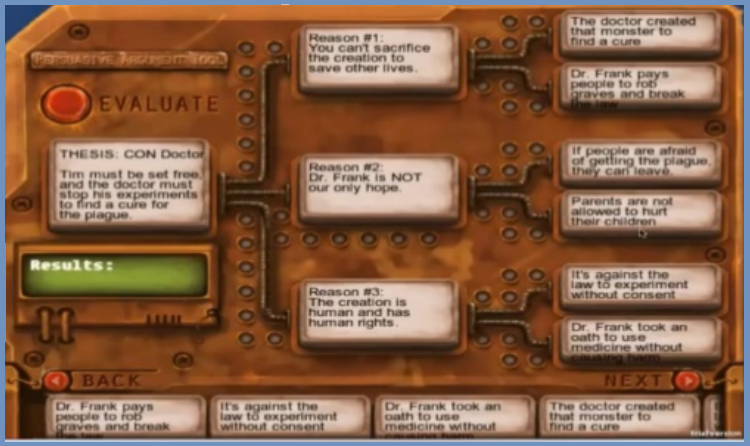
\includegraphics[scale=0.5]{Figures/atlantis}
\caption{Example (Quest Atlantis) of an Educational Game}
\end{figure}

\noindent According to Annetta (2008), the movement for the inclusion of digital games to be used in teaching and training environments first started in 2003, two years after the field of ludology, the study of games, began to gain traction in academic literature. This initiative is what started the concept of a serious game as one that can be used in an academic sense to relay information. After this point in time, various examples of serious games were made for purely academic study purposes and had found a very large use in simulation for use as explanation aides and medical training.
\\\\
The use of games as simulations may stretch the colloquial definition of a video game but in academic terms, this is one facet of video games. Frasca (2002) cites that simulations, such as the ones discussed above, can fall into one of two categories, namely; Paidea (play) and Ludus (game). “Play” refers to the simulations that lack any defined set of rules and conditions to meet a fixed goal while “Game” refers to a simulation that has these conditions and a user can directly, according to the predetermined rules, move towards a fixed goal (\cite{Frasca2002}).
\\\\
From the abovementioned definitions and examples, there is a loose description of what a serious game typically looks like and where it can be applied. However, the qualities needed by these games to effectively relay information has not been directly explained in any one piece of literature. There is also a lack of explanation on how these qualities can be applied to a game to result in what may be described as a serious game.

\subsection{Overview of Related Literature}
Annetta (2008) discusses multiple examples of these games, such as Discover Babylon and Quest Atlantis, that had been developed to immerse children and young adolescents in an academic environment. Further examples of the use of serious games have already had an impact on the military, medical and higher business education fields early in their conception and this trend continues to this day with most serious games being used within the medical fields specifically (\cite{Annetta2008}).
\\\\
Deshpande and Huang (2011) describe the use of games as a means of simulation for specific sections of work in physics and engineering courses as an addition to traditional teaching as it provides a relatively simple way to demonstrate certain phenomena. As such these authors discuss the simulation aspect of games rather than the narrative.
\\\\
The endeavour to create serious games has yet to reach schools due to certain criticisms about games in general which hinder the adoption of games as a means of teaching and learning (\cite{Virvou2005}).
\\\\
The study of serious games became more theoretical and discussion-based at lower levels and more applied with actual use at higher levels, with a great impact on medical fields and training. As such, there is a fair amount of theoretical research on specific aspects that relate to serious games as simulations and within ludology as a whole, but only a few mention the qualities a game needs to better present information to a user. 

\begin{figure}[H]
\centering
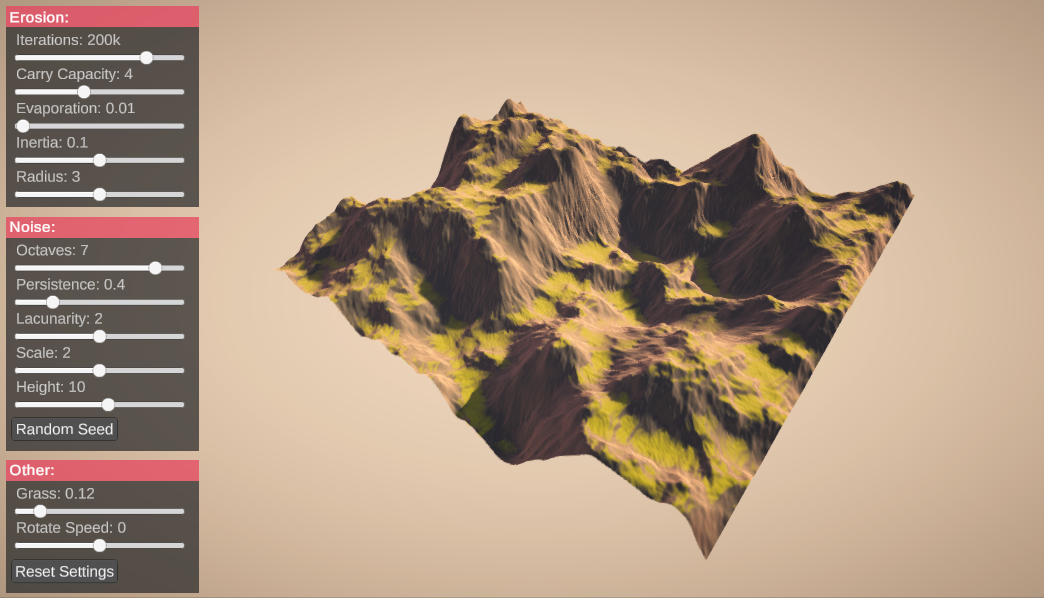
\includegraphics[scale=0.4]{Figures/soil}
\caption{Example of Using a Game to Simulate Soil Erosion}
\end{figure}

\subsection{Research Question and Expected Outcomes}
The main research question this project is set out to answers is; “What qualities does a video game require in order for it to be useful in relaying certain information to a user whilst still maintaining proper engagement with the user?”. The findings resulting from answering this question will be used in the development of a specific video game level that will attempt to teach users about the games various mechanics and enemy types presented. 
\\\\
The expected outcomes of this project is the aforementioned game as the artefact as well as a description of the qualities a game must exhibit to effectively relay information in an educational sense.

\section{Aims and Objectives of Project}
The primary aim of this study is to identify what qualities and principles can be applied to a video game to allow it to be used in a learning environment as a means to provide better engagement among certain students by providing an enjoyable delivery of information. 
\\\\
To effectively reach the aforementioned aim, all the following objectives will have to be met as certain objectives will benefit from the completion of others:
\begin{enumerate}
\item A literature study will need to be performed to gather information with a focus on:
\begin{enumerate}
\item Ludology, narratology and simulation to better understand the academia centred around this project;
\item Other implementations of serious games and the qualities they possess;
\item The impact and effects of games in early development as this is the main “target audience” if this project were to be implemented as well as in a more general sense;
\item Previous attempts to integrate game use in learning.
\end{enumerate}
\item Collect examples of games that employ some form of teaching 
(\textit{Where objective 1-b focuses on examples already discussed in an academic sense, this objective will make use of more informal analysis})
\end{enumerate}


\noindent The next aim of this project is to develop an artefact which will require the following objectives:
\begin{enumerate}
\item Learn and understand how to use the chosen development platform and associated environments;
\item Develop a base to build other levels/scenes off of;
\begin{enumerate}
\item Development of basic scripts needed.
\end{enumerate}
\item Create a specific scene/level within the aforementioned artefact that specialises in delivering information through various audio-visual stimuli that incorporates the principles and qualities found.
\end{enumerate}

\section{Procedures and Methods of Investigation}
\subsection{Research Paradigm and Methodology Used}
The research aspect of this project will be conducted in accordance with the interpretivist paradigm. The main undertaking of this paradigm is to understand the world and its’ various aspects according to the subjective experiences of people (\cite{kivunja2017understanding}). It is due to this reason that this project uses this paradigm as what each student requires to efficiently learn is subjective to each individual. Kivunja and Kuyini  (2017) further mention that the interpretivist paradigm makes use of subjective epistemology which allows the researcher to analyse the data, which in this project is the principles and qualities that allow for a game to be effective in a learning environment, through their individual cognitive processes. 
\\\\
Kivunja and Kuyini (2017) continue to list certain characteristics of research conducted under this paradigm typically possess. These include the understanding that the social world cannot be fully comprehended from one standpoint which is why this project makes use of various other studies in the compilation of the aforementioned principles and qualities. Another is that knowledge and its’ understanding is developed through the findings of the study itself.
\newpage
\noindent Design science is a methodology composed of using analytical techniques and can be used according to many paradigms to perform research in the information systems field (\cite{vaishnavi2004design}). This means of research centres on the development of artefacts to better understand certain aspects through the creation of new knowledge and that assessment of an artefacts performance (\cite{vaishnavi2004design}). This methodology was chosen as it provides certain outlines that will allow for the development and analyses of the principles and qualities for a game to be used academically through the creation of such artefact incorporation these qualities into its’ design and development. 
\\\\
Design Science also provides a general structure as to how this project will be completed as shown in Figure \ref{des} below taken from Vaishnavi and Kuechler’s (2004) work. This process allows for the development of an artefact alongside the collection of information and knowledge that can be incorporated into the design and development of the artefact as well as the evaluation of the implementation of the qualities onto the artefact. In  this case, the artefact will take the form of an article.

\begin{figure}[H]
\centering
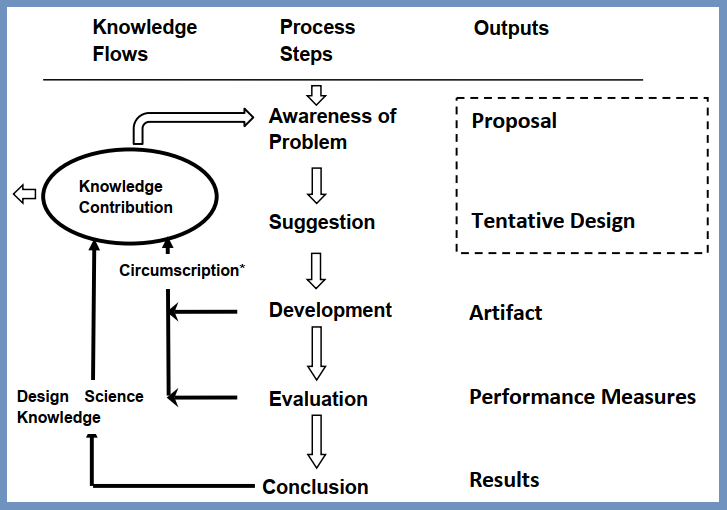
\includegraphics[scale=0.6]{Figures/ds}
\caption{The Design Science Research Process (\cite{vaishnavi2004design})}
\label{des}
\end{figure}

\subsection{Collection of Data}
This project will collect data in the form of literary studies and real-world examples of serious and educational games. The main channel of processing this data will be in the form of a literature review and consequential implementation of the findings in an article.

\subsection{Development of Artefact}
The artefact that will be developed as a part of this project will be a computer video game that will be developed as a group effort. This game will be a standalone artefact with no major links to each group members research – it may, however, be influenced by them. Due to the expansive nature of game design, the Agile software development life cycle will be used. Following this cycle of development allows for the artefact to be developed in smaller increments through the use of iterative cycles and regular meetings about the design and features of the artefact (\cite{highsmith2001agile}). According to Highsmith and Cockburn (2001), Agile also allows for “dynamic prioritisation” which allows for the shifting of development to other aspects if they urgently require more attention over others on short notice. Agile also makes use of constant testing which ensures that defects and issues are found and dealt with quickly (\cite{highsmith2001agile}). Most importantly, the development of the artefact will be continuous from the start date and will make use of weekly scrums, or discussion-based meetings on what should be developed, to ensure a regular flow of development on the game.

\subsection{Integration with Other Projects}
The development of an artefact as part of this project is being conducted alongside two other students, one focusing on the different effects on cognition from various genres and the other dealing with the controls of games. These other projects are conducted by:
\begin{itemize}
\item GC Wehmeyer (29977339)
\item Rickus Trollip (30083575)
\end{itemize}
These other projects only integrate with this one when concerning the artefact that will be developed as each will conduct a fully indecent research study and, if applicable, develop any other questionnaires or models independently. The development of the artefact will be done as a group effort and as such the computer game that will be developed for this project may be impacted by the findings of these other projects.
\pagebreak
\section{Approach to Project Management and Project Plan}
\subsection{Provisional Project Plan}
The provisional project plan is discussed below and specific dates of completion may shift due to unforeseen circumstances. This project began on the 15th of February 2021 and will be fully completed by the 8th of November 2021. During this period the project has certain deadlines for particular deliverables that will need to be adhered to. 

\begin{enumerate}
\item The first of these is the project planning and research proposal which must be completed and submitted by the 18th of April 2021. The research proposal will cover a substantiation of the project and its feasibility. The project planning includes a project description with the research question, the main aims and objectives of the project, a detailed explanation of the developmental process of the project, and a description of what will be used in the development of the project.

\item Following this, a literature study regarding Ludology as a whole, implementations of serious games, the qualities they possess, the impact and effects of games and previous attempts to integrate game use in learning. This literature review is set to be completed for submission by the 13th of June 2021. 

\item The next deliverable for this project is the demonstration of the artefact and the development of a video presentation on the 1st of November 2021. This deliverable will be met by continuously developing the artefact according to provisional dates shown in Figure 4 below. 

\item The final deliverable is the final documentation of the entire project that consists of all previous deliverables as one document with certain additions. This deliverable must be completed and submitted by the 8th of November 2021.
\end{enumerate}

\noindent A more detailed breakdown of the project plan is presented in Figure 4 below with provisional dates for the deliverables and the anticipated objectives required to meet them.


\begin{figure}[H]
\centering
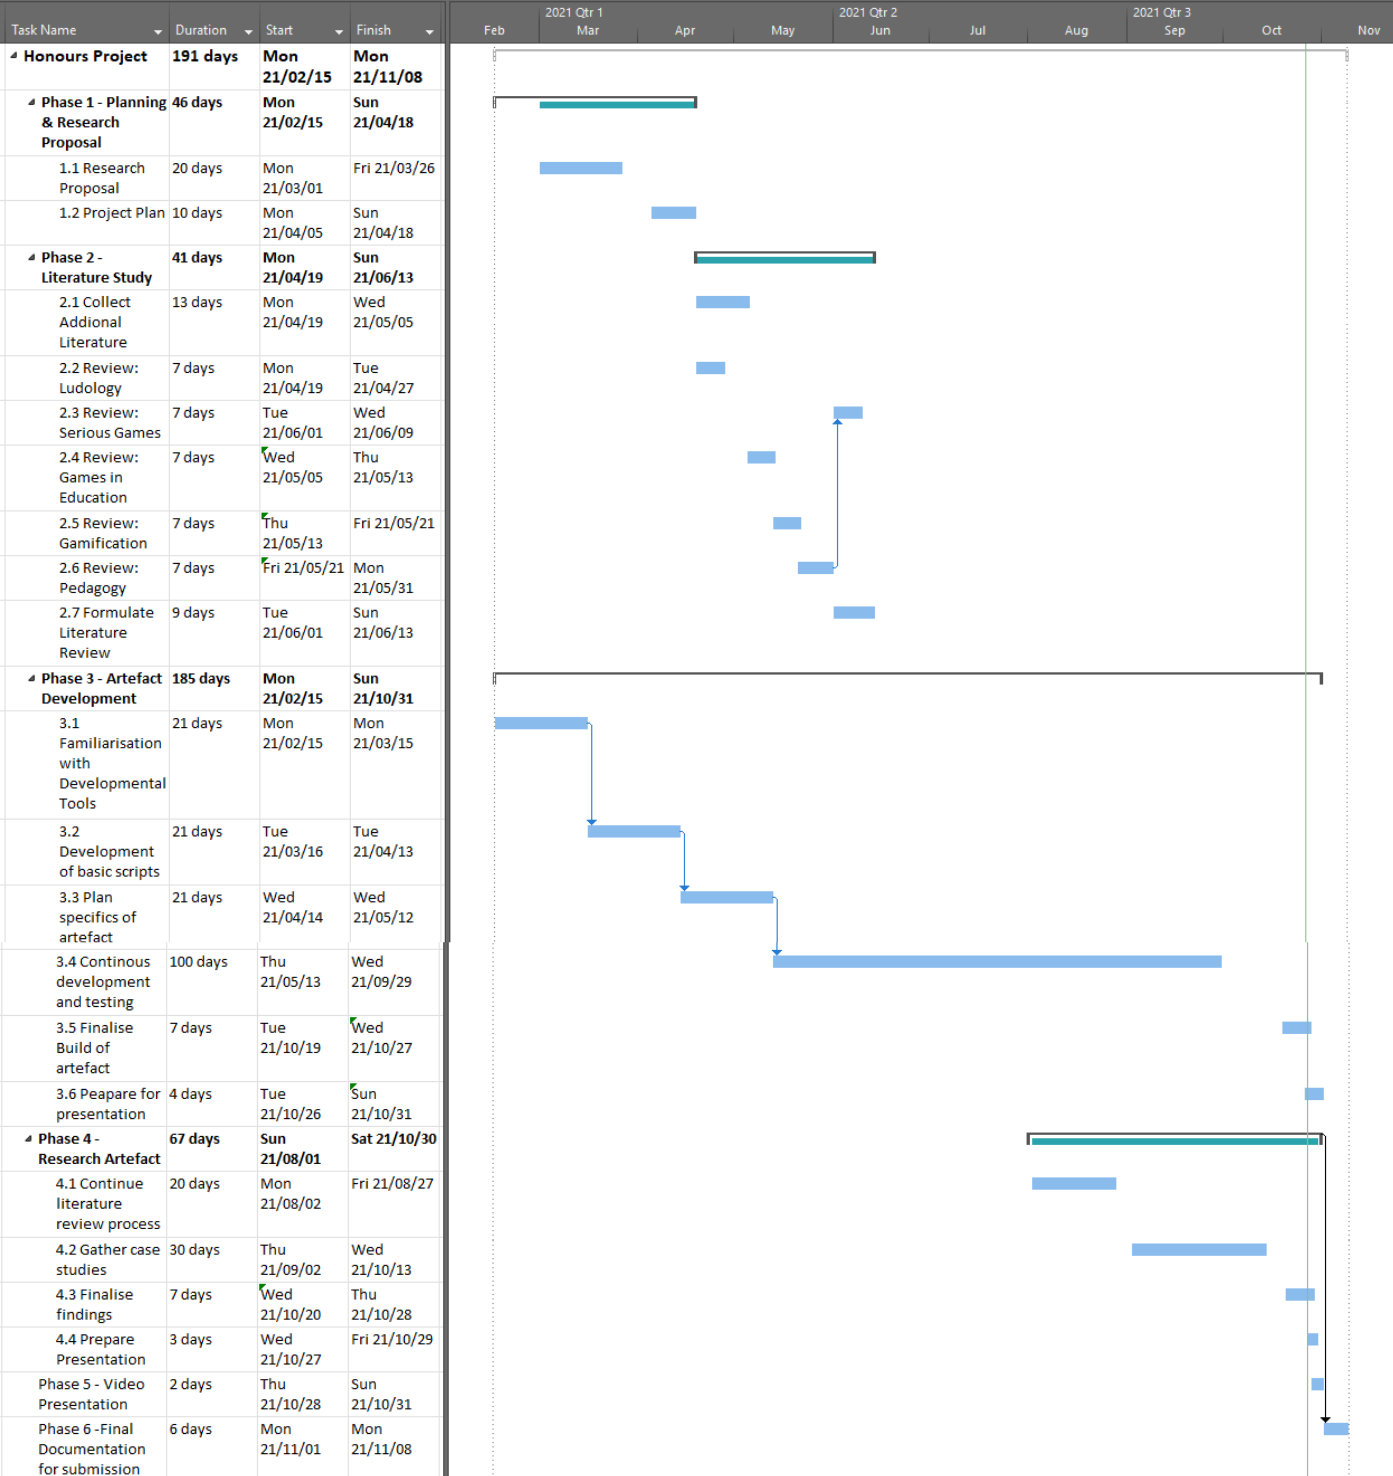
\includegraphics[scale=0.75]{Figures/gantt}
\caption{Provisional Project Plan}
\end{figure}

\subsection{Scope}
This project is split into two distinct parts. First is the research aspect that will be conducted individually which involves the review and analysis of literature and examples of serious games. This aspect aims to find and describe the qualities and principles that could allow a game to be used in a learning environment.
\\\\
The second aspect of this project is the development of a computer game as the artefact. This artefact will be developed as a group effort with each member focusing on specific areas of development and all members having some contribution to other areas.

\subsection{Limitations}
The most notable limitation towards this project is that it must be completed according to a fixed time frame which is provisionally set out as follows:
\begin{itemize}
\item Submission of the project plan and research proposal on 18th April 2021
\item Submission of the literature study on 13th June 2021
\item Demonstration of the artefact and a poster on 1st November 2021
\item Submission of the complete documentation of the project on 8th November 2021
\end{itemize}
Other time constraints will be applied according to certain aspects of development, such as meetings or self-imposed deadlines, which can only be set at a later date.
\\\\
As will be discussed in 1.6, the artefact will make use of third party resources and as such is limited to what is publicly available at no cost as not to apply any financial constraints on the projects involved with the artefact.
\\\\
Since the artefact developed is a digital computer game, the demonstration and development of it will require a system that meets the requirements for the associated development platform and environments. As such the artefact is limited to systems with the following minimum requirements - as described by Unity:
\begin{itemize}
\item Windows 7;
\item Processor with x64 architecture;
\item A capable graphics processing system with DX10, DX11 and DX12 functionality.
\end{itemize}
\pagebreak
\subsection{Risks and SWOT Analysis}
The project will have risks associated with the artefact, which will be discussed below.
\\\\
Firstly, is the risk of scope creep. As the planning only depicts and describes the basic structure and aims of the project, once development on the artefact begins the specifications and features may continue to increase in number which may cause the project to fail expectations set. As such, the intended features of the artefact should be discussed and solidified early on in its’ development to mitigate this specific risk.
\\\\
The artefact's development and the research aspect of this project is also at risk of unforeseen events. In an attempt to mitigate the harm that may be caused by these events, the artefact is being developed in such a manner to facilitate both contact sessions as well as fully digitally.

\begin{figure}[H]
\centering
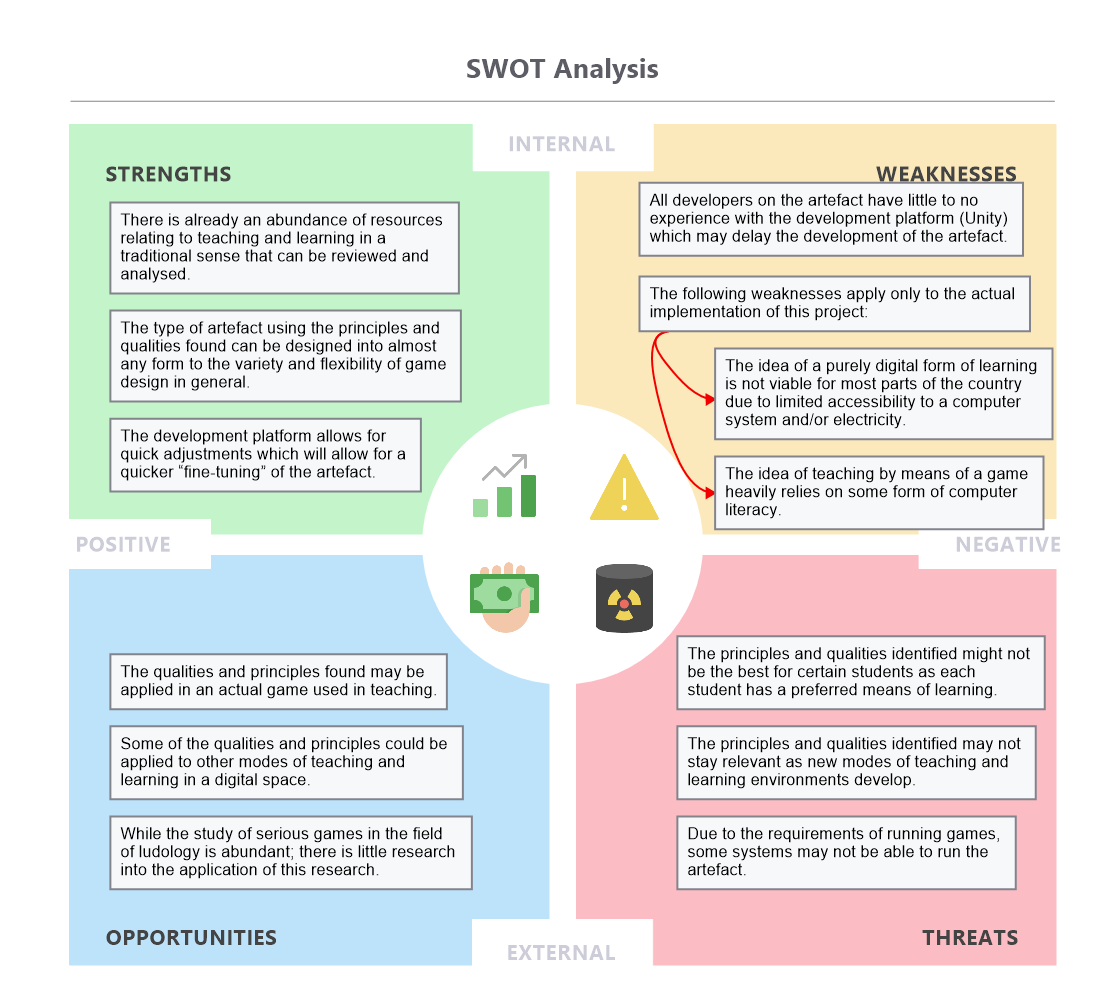
\includegraphics[scale=2]{Figures/swot}
\caption{Swot Analysis of the Project}
\end{figure}

\subsection{Contributions of Each Group Member}
This project has an element of group work as the artefact that will be developed will be done as a group. Each member of the group will be responsible for different aspects of the development of the artefact such as, but not limited to;
\begin{itemize}
\item focusing on the animation of models, 
\item development of character controls, 
\item developing a simple artificial intelligence for the enemy characters;
\item narrative design and 
\item level layout and design. 
\end{itemize}
Members may be fully responsible for the contribution of the aforementioned areas while other aspects may be worked on by all members concurrently. The specific areas that a group member will contribute towards will be discussed when the artefact begins proper and continuous development.
\\\\
However, it should be noted that each member is still solely responsible for their individual research study project that may directly or indirectly link to the artefact.

\section{Development Platform, Resources and Environments}
\subsection{Development Platform}
The main platform for the development of the artefact will be the Unity game editor developed by Unity Technologies. The 2019.4.22f version of the program will be used as it is marked as one of the publicly availably versions that is depicted to get long term support and as such should provide a fair balance of features and stability required for the development of this artefact. Unity is also equipped with various tools for the development of games, such as Probuilder which allows for the construction and editing of basic three-dimensional objects and will also be included in the development of the artefact. Other tools provided by Unity may also be employed in the development of the artefact as they become needed. Unity was chosen for the development of the artefact as it is a fairly popular game development platform and as such has a fair amount of introductory courses and tutorials on its’ use. 
\\\\
GitHub will be used in the development of the artefact to allow for a simplified way to quickly share any changes made to the artefact and track the contributions towards the artefact's development by all members involved. Hence, a repository for the artefact's files will be initialised and then used throughout its’ development life cycle. A programmer can quickly download (pull) and upload (push/commit) their changes to a project with this platform. The desktop client GitHub is used to facilitate all the operations discussed above. GitHub’s repository features will be used for the ease it provides in communicating changes between the various developers of the artefact. 
\\\\
Other development platforms may be used in the development of the artefact if they are required. One such example of this is Blender, a 3D modelling program that allows for the creation of three-dimensional objects and models and may be used if need be in the editing of models used. As such other programs currently not specified may be used for the artefact's development; specifically, in areas that Unity does not directly cater for.

\subsection{Resources}
The Unity Asset Store will be used to acquire 3D models to be used within the artefact to complete the artefact within the given time frame since this is one aspect of game development that is very time-consuming. In a similar vein, Mixamo.com will be used to acquire animations for the artefact as this is another time-consuming process.
\\\\
A list of all resources used will be compiled and the relevant creators and/or distributors will be referenced in the artefacts final documentation.  

\subsection{Environments}
Microsoft's Visual Studio IDE will be used for the creation and development of most of the scripts and classes that will be implemented into the Unity game editor. This specific IDE was chosen as it has some basic integration with the Unity editor and can be installed directly from and during the Unity editor's initial installation.

\section{Ethical Implications of Project}
This project will not make use of external participants in a formal manner that would require any ethical implications as the only participants towards the development of this projects is the developers working on the artefact itself. The prescribed ethics form has been completed and attached.


\section{Provisional Chapter Division}
This document will contain a bulk of the final project documentation and the associated literature study. It will be divided into separate chapters which are listed below with a brief description of the respective content.
\\\\
\indent \textbf{Chapter 1: Introduction} \\	
The problem that is being researched, the qualities of games needed for use in education, is discussed in Chapter 1. Information on the background of this problem, similar research and the research contribution will be discussed. Furthermore, the aim of the study in addition to the planned method of conduct will be discussed.
\\
\indent \textbf{Chapter 2: Literature Study} \\
Chapter 2 will discuss the impact of games both in early development and in general in more detail, the accessibility of games as well as a focus on games being used in learning. It will attempt to find what qualities and principles work best to make a game a suitable means of learning.
\\
\indent \textbf{Chapter 3: Development of Artefact and Article} \\
The accompanying artefact that will be developed as a part of the study will be discussed along with the development process of the article.
\\
\indent \textbf{Chapter 4: Results} \\
A discussion on the results obtained will be presented in this chapter. This chapter will focus on the main use of the artefact and the qualities an educational game needs.
\\
\indent \textbf{Chapter 5: Reflection} \\
The contents and results of the study will be briefly discussed and reiterated in an overview in addition to a brief discussion on how the project could possibly progress.
\\
\indent \textbf{Reference List} \\
Contains all literary works referenced in the project.

